% Oorka whitepaper. Self-contained: all figures are TikZ / pgfplots. Compile with pdfLaTeX (Overleaf default).
\documentclass[11pt,a4paper]{article}

% ---------------------------------------------------------------- packages
\usepackage[T1]{fontenc}
\usepackage[utf8]{inputenc}
\usepackage{lmodern}
\usepackage[margin=2.4cm]{geometry}
\usepackage{microtype}
\usepackage{amsmath,amssymb,amsthm}
\usepackage{booktabs,tabularx,array}
\usepackage{enumitem}
\usepackage[dvipsnames]{xcolor}
\usepackage{tikz}
\usetikzlibrary{arrows.meta,positioning,shapes.geometric,shapes.misc,fit,backgrounds,calc,patterns,decorations.pathreplacing}
\usepackage{pgfplots}
\pgfplotsset{compat=1.18}
\usepackage{caption}
\usepackage{float}
\usepackage{algorithm}
\usepackage{algpseudocode}
\usepackage{fancyhdr}
\usepackage{titlesec}
\usepackage[hidelinks]{hyperref}

% ---------------------------------------------------------------- style
\definecolor{ink}{HTML}{1B2430}
\definecolor{ink2}{HTML}{55606E}
\definecolor{accent}{HTML}{2C8C7A}
\definecolor{amber}{HTML}{C8871A}
\definecolor{violet}{HTML}{7B4FC9}
\definecolor{rose}{HTML}{C24B5A}
\definecolor{bench}{HTML}{8A96A3}
\definecolor{paper}{HTML}{F4F6F8}

\hypersetup{colorlinks=true,linkcolor=accent,citecolor=accent,urlcolor=accent}
\captionsetup{font=small,labelfont={bf,color=ink},textfont={color=ink2}}
\titleformat{\section}{\Large\bfseries\color{ink}}{\thesection}{0.8em}{}
\titleformat{\subsection}{\large\bfseries\color{ink}}{\thesubsection}{0.7em}{}
\setlist{itemsep=2pt,topsep=4pt}

\pagestyle{fancy}
\fancyhf{}
\fancyhead[L]{\small\color{ink2}Oorka: Contested Liquidity Curation on Uniswap v4}
\fancyhead[R]{\small\color{ink2}\thepage}
\renewcommand{\headrulewidth}{0.3pt}

\newtheorem{definition}{Definition}
\newtheorem{proposition}{Proposition}

\newcommand{\code}[1]{\texttt{\small #1}}
\newcommand{\Lv}{L^{\mathrm{v}}}
\newcommand{\NAV}{\mathrm{NAV}}
\newcommand{\Q}{2^{128}}

% shared TikZ styles
\tikzset{
  box/.style={draw=ink,rounded corners=3pt,fill=white,align=center,font=\small,inner sep=6pt,minimum height=1.0cm},
  core/.style={box,fill=accent!12,draw=accent,thick},
  actor/.style={box,fill=paper},
  ext/.style={box,fill=violet!8,draw=violet},
  arr/.style={-{Stealth[length=2.4mm]},thick,color=ink},
  darr/.style={arr,dashed},
  lbl/.style={font=\scriptsize,color=ink2,fill=white,inner sep=1.5pt},
  decision/.style={diamond,aspect=2.2,draw=ink,fill=amber!10,font=\small,align=center,inner sep=1pt},
  proc/.style={rectangle,rounded corners=3pt,draw=ink,fill=white,font=\small,align=center,minimum width=4.6cm,minimum height=0.85cm},
  term/.style={rounded rectangle,draw=accent,fill=accent!12,thick,font=\small\bfseries,minimum width=3.2cm,minimum height=0.8cm},
}

% ---------------------------------------------------------------- title
\title{%
  \vspace{-1.2cm}
  {\color{accent}\rule{\linewidth}{1.2pt}}\\[0.6em]
  {\Huge\bfseries\color{ink} Oorka}\\[0.4em]
  {\Large\color{ink} Contested Liquidity Curation on Uniswap~v4}\\[0.3em]
  {\normalsize\color{ink2} Making LP vault managers earn the seat with measured, on-chain performance}\\[0.2em]
  {\color{accent}\rule{\linewidth}{1.2pt}}
}
\author{Debojyoti De Majumder\\{\small\color{ink2}oorka.djyo.tech \textperiodcentered{} oorkadocs.djyo.tech}}
\date{\small November 2026 \textperiodcentered{} Draft v1.0 \textperiodcentered{} \href{https://github.com/debojyoti10CC/oorka}{github.com/debojyoti10CC/oorka}}

\begin{document}
\maketitle
\thispagestyle{empty}

\begin{abstract}
\noindent
Curated liquidity vaults ask depositors to trust a manager whose skill cannot be verified on-chain and who is hard to replace. We present \textbf{Oorka}, a Uniswap~v4 hook that turns the manager seat of a concentrated-liquidity vault into a continuous, self-settling competition. Any strategist can challenge the incumbent by posting a bond and declaring a price range. The hook places a dust-sized \emph{probe position} at every declared range. This forces the PoolManager to track fee growth at exactly those ticks, so each strategy's performance is measured from real swap flow, with no oracle, no off-chain backtest and no capital at risk. Each curator holds a virtual \emph{paper portfolio} that is marked to a manipulation-resistant reference price. A challenger who beats the incumbent by a margin for a configurable number of consecutive epochs takes the seat. The vault's real liquidity then migrates to the winner's range in the same transaction, and part of the deposed manager's bond is paid to depositors. A passive \emph{benchmark} portfolio is scored alongside the curators, so every epoch reports on-chain whether active management beat doing nothing. The seat holder is paid a performance fee only on value created above the benchmark and the vault's high-water mark. Settlement prices use a time-weighted average of block-open ticks that the hook builds itself. Donations, which would inflate fee growth without trading, are rejected. Settlement is automated without off-chain keepers via Reactive Network: an event-driven reactive contract, \emph{Oorka Pulse}, watches the pool's own swaps and settles each epoch seconds after it ends, with a CRON timer as fallback. The system is deployed on Unichain Sepolia, with its reactive contract on Reactive Lasna. Auction-managed AMMs sell the manager seat to the highest bidder; Oorka makes curators \emph{earn} it.
\end{abstract}

\vspace{0.4em}
\noindent\fcolorbox{accent}{accent!6}{\parbox{\dimexpr\linewidth-2\fboxsep-2\fboxrule}{\small
\textbf{Contributions.}
(1)~\emph{Probe positions}: a technique that uses dust liquidity and \code{getFeeGrowthInside} to measure what any hypothetical range earns, under live order flow.
(2)~A \emph{contested curation} mechanism: epochs, margins, win streaks, bonded challengers, automatic liquidity migration and slashing.
(3)~An on-chain \emph{benchmark report} that compares the vault with a passive range every epoch, and a \emph{benchmark-relative performance fee} with a high-water mark that pays the manager only for real outperformance.
(4)~A \emph{manipulation-resistant pricing layer}: block-open pricing for accounting, a hook-built epoch TWAP for settlement, and rejection of \code{donate()}.
(5)~\emph{Event-driven, keeper-free settlement}: Oorka Pulse reacts to the pool's swaps and the hook's events through Reactive Network and settles within seconds of an epoch boundary, with a CRON fallback.
(6)~A \emph{live testnet deployment} on Unichain Sepolia and Reactive Lasna, with a public dashboard.
}}

\tableofcontents
\newpage

% ====================================================================
\section{Introduction}
Concentrated liquidity~\cite{univ3} turned liquidity provision into an active strategy. Where an LP places capital, and when it moves it, decides whether fee income outruns adverse selection and loss-versus-rebalancing~\cite{lvr}. Most LPs therefore delegate to vaults run by a manager (a \emph{curator}). The trust model of these vaults has barely changed:

\begin{itemize}
  \item \textbf{Selection is off-chain.} Depositors pick managers based on marketing, or on backtests the manager ran on data the manager chose.
  \item \textbf{Performance is not comparable.} No on-chain record shows whether this manager beats the alternatives \emph{under the same order flow, right now}.
  \item \textbf{Replacement is costly.} Removing an under-performing manager takes governance or a full withdrawal, which realises slippage and gas for every depositor.
\end{itemize}

Uniswap~v4 hooks~\cite{univ4} let a pool run custom logic around swaps and liquidity changes. Active liquidity management usually splits into three separate problems: curating strategists, measuring their strategies, and migrating capital between them. Oorka treats these as one mechanism rather than three features: \emph{measure} every candidate strategy on live flow, \emph{select} the manager by measured performance, and \emph{migrate} the vault automatically when the measurement says so.

\paragraph{Positioning.} Auction-managed AMMs (am-AMM)~\cite{amamm}, and the hooks that implement them (e.g.\ Chronus, Maestro, Turnstile in public hook directories~\cite{uhidir}), also contest a manager role, but they \emph{sell} it: the seat goes to whoever pays the most rent. Oorka allocates the seat by \emph{demonstrated LP performance}, and depositors can audit every input to that decision on-chain.

% ====================================================================
\section{Background}
\subsection{Fee growth in concentrated liquidity}
A Uniswap pool tracks a global fee growth per unit of liquidity, $g_{\text{global}}$, one value per token, in Q128 fixed point. Each initialized tick stores the fee growth on its far side, $g_{\text{out}}$. For a range $[t_\ell, t_u)$, the fee growth inside is
\begin{equation}
  g_{\text{in}}(t_\ell,t_u) = g_{\text{global}} - g_{\text{below}}(t_\ell) - g_{\text{above}}(t_u),
\end{equation}
and a position with liquidity $L$ accrues $\Delta g_{\text{in}} \cdot L / \Q$ in fees between two observations. The key constraint for Oorka is that \emph{$g_{\text{out}}$ only exists for initialized ticks}: a tick nobody has liquidity at has no fee history. A hypothetical range therefore cannot be measured after the fact.

\subsection{Uniswap v4 hooks}
In v4 a single \code{PoolManager} holds every pool. A hook is a contract whose address bits say which callbacks it implements (e.g.\ \code{beforeSwap}). A hook can also act as a liquidity provider in its own pool through the \code{unlock} callback, owning positions identified by \code{(owner, tickLower, tickUpper, salt)}. Oorka uses both: callbacks for pricing and safety, and hook-owned positions for probes and for the vault.

% ====================================================================
\section{System overview}
Figure~\ref{fig:arch} shows the components. One contract, \code{OorkaHook}, is the v4 hook, the vault (ERC-20 shares), and the curator registry.

\begin{figure}[h]
\centering
\resizebox{\linewidth}{!}{%
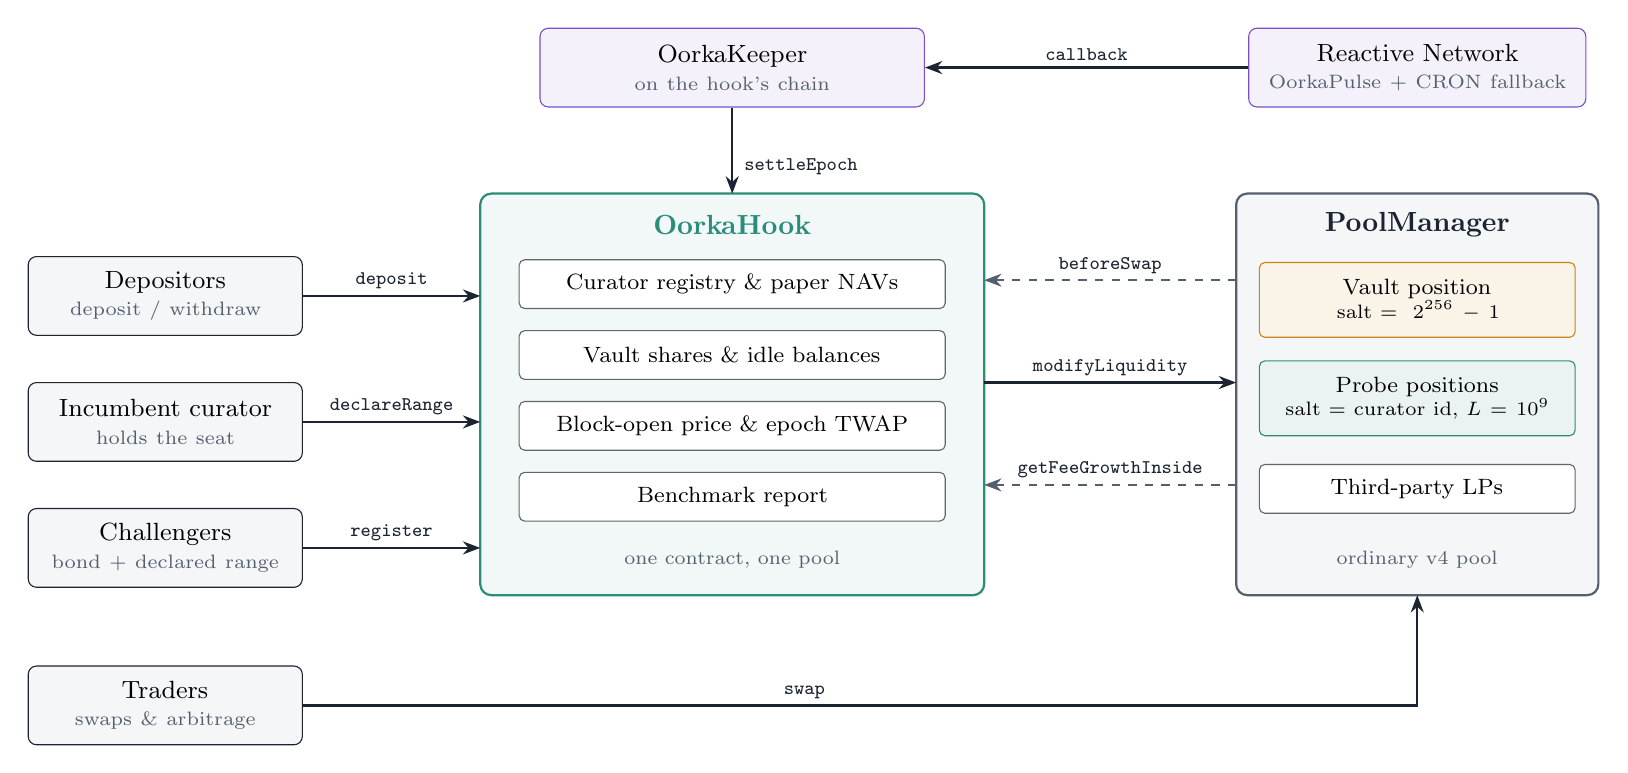
\begin{tikzpicture}[
    x=1cm,y=1cm,
    mod/.style={draw=ink!70,rounded corners=2pt,fill=white,font=\footnotesize,align=center,text width=5.2cm,minimum height=0.62cm,inner sep=3pt},
    cellbox/.style={mod,text width=3.8cm},
    act/.style={draw=ink,rounded corners=3pt,fill=paper,font=\small,align=center,text width=3.2cm,minimum height=1.0cm,inner sep=4pt},
    sub/.style={font=\scriptsize\color{ink2}},
    flow/.style={-{Stealth[length=2.2mm]},thick,color=ink},
    rflow/.style={flow,dashed,color=ink2},
    elbl/.style={font=\scriptsize\ttfamily,color=ink,above,inner sep=2pt},
  ]
  % ---------------- containers (hook: x 3.4..9.8, pool manager: x 13.0..17.6)
  \draw[accent,thick,rounded corners=4pt,fill=accent!6] (3.4,-1.4) rectangle (9.8,3.7);
  \node[font=\bfseries\color{accent}] at (6.6,3.3) {OorkaHook};
  \draw[ink2,thick,rounded corners=4pt,fill=paper] (13.0,-1.4) rectangle (17.6,3.7);
  \node[font=\bfseries\color{ink}] at (15.3,3.3) {PoolManager};

  % ---------------- hook modules
  \node[mod] at (6.6,2.55) {Curator registry \& paper NAVs};
  \node[mod] at (6.6,1.65) {Vault shares \& idle balances};
  \node[mod] at (6.6,0.75) {Block-open price \& epoch TWAP};
  \node[mod] at (6.6,-0.15) {Benchmark report};
  \node[sub] at (6.6,-0.95) {one contract, one pool};

  % ---------------- pool manager positions
  \node[cellbox,minimum height=0.95cm,fill=amber!10,draw=amber] at (15.3,2.35) {Vault position\\[-1pt]{\scriptsize salt $=2^{256}-1$}};
  \node[cellbox,minimum height=0.95cm,fill=accent!10,draw=accent] at (15.3,1.1) {Probe positions\\[-1pt]{\scriptsize salt $=$ curator id, $L=10^{9}$}};
  \node[cellbox] at (15.3,-0.05) {Third-party LPs};
  \node[sub] at (15.3,-0.95) {ordinary v4 pool};

  % ---------------- actors (right edge at x = 1.2)
  \node[act] (dep) at (-0.6,2.4)  {Depositors\\[-1pt]{\scriptsize\color{ink2} deposit / withdraw}};
  \node[act] (inc) at (-0.6,0.8)  {Incumbent curator\\[-1pt]{\scriptsize\color{ink2} holds the seat}};
  \node[act] (cha) at (-0.6,-0.8) {Challengers\\[-1pt]{\scriptsize\color{ink2} bond + declared range}};
  \node[act] (trd) at (-0.6,-2.8) {Traders\\[-1pt]{\scriptsize\color{ink2} swaps \& arbitrage}};

  % ---------------- automation row
  \node[act,fill=violet!8,draw=violet,text width=4.6cm] (kp) at (6.6,5.3) {OorkaKeeper\\[-1pt]{\scriptsize\color{ink2} on the hook's chain}};
  \node[act,fill=violet!8,draw=violet,text width=4.0cm] (rn) at (15.3,5.3) {Reactive Network\\[-1pt]{\scriptsize\color{ink2} OorkaPulse $+$ CRON fallback}};

  % ---------------- edges: actors -> hook
  \draw[flow] (dep.east) -- node[elbl]{deposit}      (3.4,2.4);
  \draw[flow] (inc.east) -- node[elbl]{declareRange} (3.4,0.8);
  \draw[flow] (cha.east) -- node[elbl]{register}     (3.4,-0.8);

  % ---------------- edges: hook <-> pool manager
  \draw[rflow] (13.0,2.6) -- node[elbl]{beforeSwap}         (9.8,2.6);
  \draw[flow]  (9.8,1.3)  -- node[elbl]{modifyLiquidity}    (13.0,1.3);
  \draw[rflow] (13.0,0.0) -- node[elbl]{getFeeGrowthInside} (9.8,0.0);

  % ---------------- edges: traders and automation
  \draw[flow] (trd.east) -- node[elbl,pos=0.45]{swap} (15.3,-2.8) -- (15.3,-1.4);
  \draw[flow] (rn.west) -- node[elbl]{callback} (kp.east);
  \draw[flow] (kp.south) -- node[elbl,right,xshift=2pt,yshift=-6pt]{settleEpoch} (6.6,3.7);
\end{tikzpicture}}
\caption{Architecture. The hook owns two kinds of positions inside the PoolManager, separated by salt. The vault position holds real depositor capital at the incumbent's range. Probe positions hold dust liquidity at every declared range, so the pool keeps fee history at those ticks. Reactive Network triggers settlement without an off-chain keeper.}
\label{fig:arch}
\end{figure}

\paragraph{Roles.}
\begin{itemize}
  \item \textbf{Depositors} supply both tokens and receive vault shares. Their liquidity always sits at the incumbent's range.
  \item \textbf{Curators} register with a bond and a range. The first registrant takes the seat. Later registrants are challengers.
  \item \textbf{Traders} interact with an ordinary v4 pool. Oorka never changes swap pricing or fees.
  \item \textbf{Anyone} may call \code{settleEpoch()} once an epoch has ended. In practice OorkaKeeper does, driven by Reactive Network.
\end{itemize}

% ====================================================================
\section{Mechanism}

\subsection{Probe positions}
\begin{definition}[Probe]
For a curator $i$ with declared range $[t_\ell^i, t_u^i)$, the probe is a hook-owned position with liquidity $L_p = 10^9$, salt $= i$, and that same range.
\end{definition}

The probe's only purpose is to keep the range's boundary ticks initialized, so that $g_{\text{in}}(t_\ell^i,t_u^i)$ is maintained by the PoolManager from the moment of declaration. Its capital cost is negligible: dust amounts of both tokens, paid by the curator. It also earns its own (negligible) share of fees. Because probes are real positions, the fee growth they expose is the fee growth \emph{any} liquidity in that range would have earned under the observed order flow. That is a forward test, not a backtest.

\subsection{Paper portfolios}
Each curator holds a virtual portfolio with initial value $\NAV_0 = 1{,}000$ units of token1. At declaration the hook chooses a \emph{virtual liquidity} $\Lv_i$ so that the portfolio is worth exactly its current NAV at the reference price $\sqrt{P}$:
\begin{equation}
  \Lv_i = \NAV \cdot \frac{L_1}{V(L_1;\, t_\ell^i, t_u^i, \sqrt{P})}, \qquad L_1 = 10^{18},
\end{equation}
where $V(L; t_\ell, t_u, \sqrt P)$ is the token1 value of the token amounts a position of liquidity $L$ holds at price $P$. Between observations the portfolio accrues
\begin{equation}
  f_k = \frac{\big(g^{(k)}_{\text{in}}(t) - g^{(k)}_{\text{in}}(t_{\text{last}})\big)\cdot \Lv_i}{\Q}, \qquad k\in\{0,1\},
\end{equation}
with modular (wrapping) subtraction, as in Uniswap's own accounting. The NAV at price $P$ is
\begin{equation}
  \NAV_i(P) = \underbrace{x_i(P)\,P + y_i(P)}_{\text{position at }P} \;+\; \underbrace{(c_0 + f_0)\,P + (c_1 + f_1)}_{\text{collected and pending fees}},
\end{equation}
where $(x_i, y_i)$ are the token amounts of $\Lv_i$ in the range at $P$, and $c_k$ is fee cash already marked. The NAV therefore includes both \emph{real fee income} and \emph{real price exposure} (impermanent loss) of the declared range.

\paragraph{Range changes.} When a curator moves to a new range, the portfolio is first charged a switch cost of $s$ basis points, a proxy for real rebalancing slippage and fees. It is then re-derived at the new range with $\NAV' = \NAV\,(1 - s/10^4)$. The epoch baseline is unchanged, so the cost shows up in the score.

\subsection{Epochs, scoring and takeover}
Time is divided into epochs of length $T$. At settlement each active portfolio $i$ is scored by its epoch growth
\begin{equation}
  G_i = \frac{\NAV_i(\bar P)}{\NAV_i^{\text{start}}},
\end{equation}
where $\bar P$ is the settlement price (Section~\ref{sec:pricing}). Let $h$ be the incumbent. A challenger $i$ \emph{wins} the epoch if it was present for the whole epoch and
\begin{equation}
  G_i > G_h \left(1 + \frac{m}{10^4}\right),
\end{equation}
with margin $m$ in basis points. Wins accumulate into a streak, and a loss resets the streak to zero. When at least one challenger's streak reaches $W$, the one with the highest $G_i$ takes the seat. Figure~\ref{fig:settle} gives the full procedure.

\begin{figure}[p]
\centering
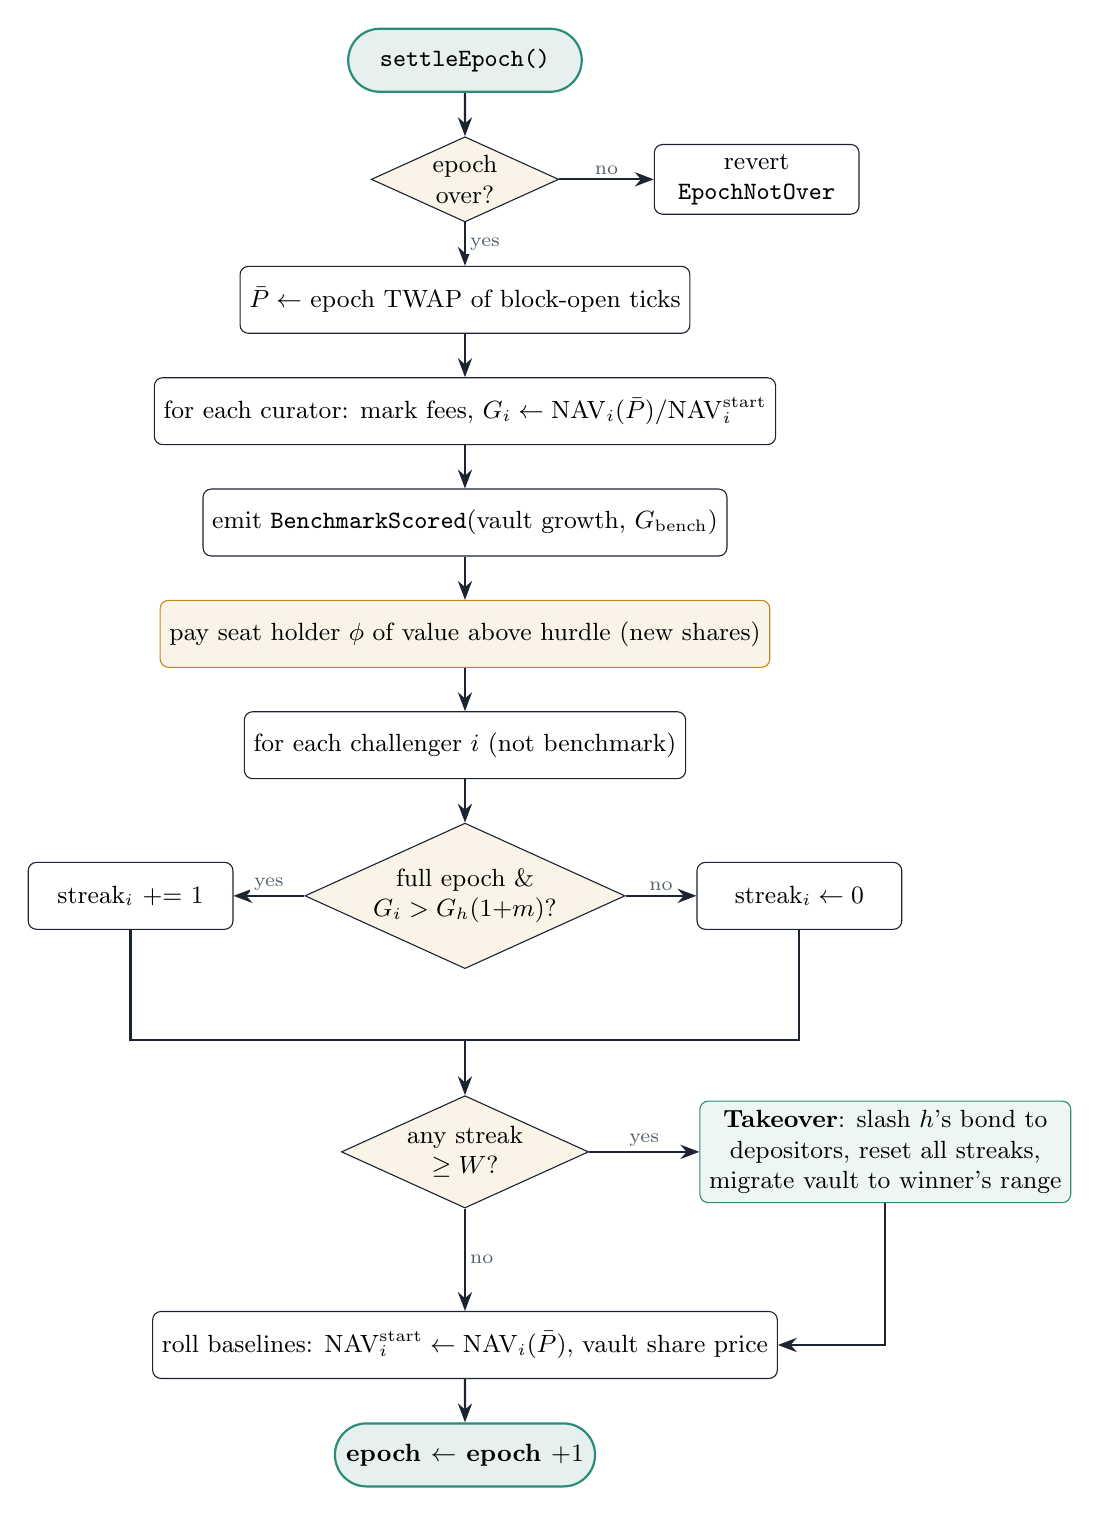
\begin{tikzpicture}[node distance=0.55cm]
  \node[term] (s) {\code{settleEpoch()}};
  \node[decision,below=of s] (d1) {epoch\\over?};
  \node[proc,right=1.2cm of d1,minimum width=2.6cm] (r1) {revert\\\code{EpochNotOver}};
  \node[proc,below=of d1] (p) {$\bar P \leftarrow$ epoch TWAP of block-open ticks};
  \node[proc,below=of p] (m) {for each curator: mark fees, $G_i \leftarrow \NAV_i(\bar P)/\NAV_i^{\text{start}}$};
  \node[proc,below=of m] (b) {emit \code{BenchmarkScored}(vault growth, $G_{\text{bench}}$)};
  \node[proc,below=of b,fill=amber!10,draw=amber] (fee) {pay seat holder $\phi$ of value above hurdle (new shares)};
  \node[proc,below=of fee] (l) {for each challenger $i$ (not benchmark)};
  \node[decision,below=of l] (d2) {full epoch \&\\$G_i > G_h(1{+}m)$?};
  \node[proc,left=0.9cm of d2,minimum width=2.6cm] (w) {streak$_i$ += 1};
  \node[proc,right=0.9cm of d2,minimum width=2.6cm] (z) {streak$_i \leftarrow 0$};
  \node[decision,below=1.6cm of d2] (d3) {any streak\\$\ge W$?};
  \coordinate (join) at ($(d3.north)+(0,0.7)$);
  \node[proc,right=1.4cm of d3,minimum width=4.2cm,fill=accent!8,draw=accent] (t) {\textbf{Takeover}: slash $h$'s bond to\\depositors, reset all streaks,\\migrate vault to winner's range};
  \node[proc,below=1.3cm of d3] (roll) {roll baselines: $\NAV^{\text{start}}_i \leftarrow \NAV_i(\bar P)$, vault share price};
  \node[term,below=of roll] (e) {epoch $\leftarrow$ epoch $+1$};

  \draw[arr] (s) -- (d1);
  \draw[arr] (d1) -- node[lbl,above]{no} (r1);
  \draw[arr] (d1) -- node[lbl,right]{yes} (p);
  \draw[arr] (p) -- (m);
  \draw[arr] (m) -- (b);
  \draw[arr] (b) -- (fee);
  \draw[arr] (fee) -- (l);
  \draw[arr] (l) -- (d2);
  \draw[arr] (d2) -- node[lbl,above]{yes} (w);
  \draw[arr] (d2) -- node[lbl,above]{no} (z);
  \draw[thick,color=ink] (w.south) |- (join);
  \draw[thick,color=ink] (z.south) |- (join);
  \draw[arr] (join) -- (d3.north);
  \draw[arr] (d3.east) -- node[lbl,above]{yes} (t.west);
  \draw[arr] (t) |- (roll);
  \draw[arr] (d3) -- node[lbl,right]{no} (roll);
  \draw[arr] (roll) -- (e);
\end{tikzpicture}
\caption{Epoch settlement. The procedure is permissionless and deterministic. Every quantity it uses is readable on-chain.}
\label{fig:settle}
\end{figure}

\subsection{Liquidity migration and slashing}
On takeover the hook, inside a single \code{unlock}:
\begin{enumerate}
  \item removes the vault position and collects its fees into the vault's idle balances;
  \item computes the maximal liquidity the idle balances support at the winner's range and current spot price;
  \item adds that liquidity at the winner's range. Any unmatched remainder stays idle and is included in the share price.
\end{enumerate}
A fraction $\sigma$ of the deposed incumbent's bond moves into the vault's idle token1 balance. This directly raises the share price for depositors. All streaks reset, so wins earned against the previous incumbent cannot be carried into the new reign.

\subsection{The benchmark}
A single \emph{benchmark} portfolio can be registered per pool. It is a paper portfolio on a fixed wide range with no owner and no bond. It can never be moved, exited, or seated. At every settlement the hook emits
\[
  \code{BenchmarkScored}\big(\text{epoch},\; G_{\text{vault}},\; G_{\text{bench}}\big),
  \qquad G_{\text{vault}} = \frac{\text{share price}(\bar P)}{\text{share price at epoch start}},
\]
and \code{benchmarkReport()} exposes both growths since inception and for the running epoch. The benchmark answers the depositor's real question: \emph{does the contested seat beat sitting still?}

\subsection{Benchmark-relative performance fee}
Holding the seat must be worth competing for, but the manager should be paid only for value a passive range would not have produced. At each settlement, \emph{before} any takeover, the seat holder $h$ is paid a fraction $\phi$ of the value the vault created above a hurdle. Let $p_0$ be the share price at epoch start, $p$ the share price at $\bar P$, $p_{\text{hwm}}$ the highest share price recorded at any settlement, and $S$ the share supply. The hurdle growth is
\begin{equation}
  H = \max\!\left(1,\; G_{\text{bench}},\; \frac{p_{\text{hwm}}}{p_0}\right),
\end{equation}
so there is no fee on losses, no fee for matching the benchmark, and no fee for recovering an earlier drawdown. The fee value is
\begin{equation}
  F = \phi \cdot \max\big(0,\; p - H p_0\big)\cdot S .
\end{equation}
It is paid in \emph{newly minted vault shares}, so no tokens leave the pool. Minting $s$ shares dilutes depositors by exactly $F$ when
\begin{equation}
  \frac{s}{S + s}\,\NAV = F \quad\Longleftrightarrow\quad s = \frac{F\, S}{\NAV - F}.
\end{equation}
The hook emits \code{PerformanceFee}(epoch, curator, recipient, shares, value), then raises $p_{\text{hwm}}$ to the post-fee share price. With $\phi = 10\%$, depositors keep 90\% of every unit of outperformance, and the benchmark's own return in full.

% ====================================================================
\section{Pricing and manipulation resistance}\label{sec:pricing}
Oorka's scores are only as good as the price they are marked at. Oorka uses two prices, both derived from the pool itself.

\paragraph{Block-open price (live accounting).} On the first swap of each block, \code{beforeSwap} snapshots the pool price before that swap executes. Views, deposits and withdrawals use this price. Any action that moves vault capital (deposit, withdraw, incumbent rebalance, compound) reverts if spot deviates from the block-open tick by more than $\delta_{\max}$ ticks. An in-block push (flash swap, sandwich) therefore can neither move NAVs nor be used to enter or exit the vault at a distorted price.

\paragraph{Epoch TWAP (settlement).} The block-open snapshot alone is not enough at settlement. In a block with no swap yet, the latest price \emph{is} spot, so a price pushed at the end of block $N$ could be settled at the start of block $N{+}1$. Oorka therefore maintains a tick accumulator, updated in \code{beforeSwap}:
\begin{equation}
  C \leftarrow C + \tau_{\text{last}} \cdot (t_{\text{now}} - t_{\text{last}}), \qquad \tau_{\text{last}} \leftarrow \text{block-open tick}, \qquad t_{\text{last}} \leftarrow t_{\text{now}},
\end{equation}
and settles at the epoch's time-weighted average tick
\begin{equation}
  \bar\tau = \left\lfloor \frac{C(t_{\text{now}}) - C(t_{\text{epoch start}})}{t_{\text{now}} - t_{\text{epoch start}}} \right\rfloor, \qquad \sqrt{\bar P} = 1.0001^{\bar\tau/2}.
\end{equation}

\begin{proposition}
A price deviation $\Delta\tau$ that holds for $d$ seconds within an epoch of length $T$ shifts the settlement tick by at most $\Delta\tau\cdot d/T$ (plus one tick of rounding). A deviation pushed in block $N$ and never observed as a block-open tick before settlement contributes nothing.
\end{proposition}

\noindent With $T=1$ hour, a 12-second push of 8{,}000 ticks shifts the settlement tick by at most about 27 ticks. The test suite checks the cross-block case explicitly (Section~\ref{sec:eval}).

\begin{figure}[h]
\centering
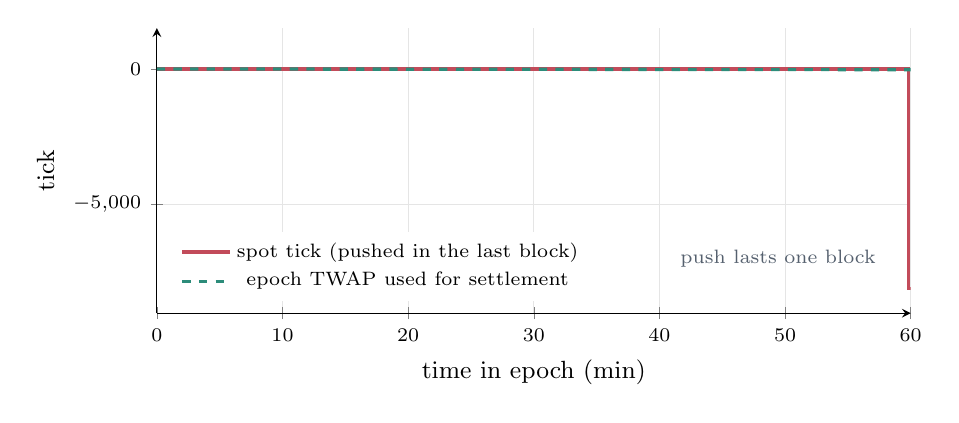
\begin{tikzpicture}
\begin{axis}[
  width=0.92\linewidth, height=5.2cm,
  xlabel={time in epoch (min)}, ylabel={tick},
  xmin=0, xmax=60, ymin=-9000, ymax=1500,
  axis lines=left, grid=major, grid style={draw=gray!20},
  legend style={draw=none,fill=white,font=\scriptsize,at={(0.02,0.04)},anchor=south west},
  tick label style={font=\scriptsize}, label style={font=\small},
  ]
  \addplot[const plot, very thick, color=rose] coordinates {(0,0) (59.8,0) (59.8,-8100) (60,-8100)};
  \addlegendentry{spot tick (pushed in the last block)}
  \addplot[very thick, color=accent, dashed] coordinates {(0,0) (60,-27)};
  \addlegendentry{epoch TWAP used for settlement}
  \node[font=\scriptsize,color=ink2,anchor=east] at (axis cs:58,-7000) {push lasts one block};
\end{axis}
\end{tikzpicture}
\caption{Why settlement uses the epoch TWAP. A last-block push moves spot by thousands of ticks, but the settlement price barely moves.}
\label{fig:twap}
\end{figure}

\paragraph{Donations.} \code{donate()} adds directly to $g_{\text{global}}$ for in-range liquidity without any swap. Narrow ranges have high $\Lv$ per unit of NAV, so a donation would inflate a tight challenger's score far more than a wide incumbent's. Oorka claims the \code{beforeDonate} permission and reverts every donation to its pool.

\subsection{Threat model}
\begin{table}[H]
\centering\small
\begin{tabularx}{\linewidth}{>{\raggedright\arraybackslash}p{5.2cm}X}
\toprule
\textbf{Attack} & \textbf{Defense} \\
\midrule
Flash-swap to inflate paper NAV before settling & NAVs are marked at block-open (live) and epoch-TWAP (settlement) prices. \\
Push the price at the end of block $N$, settle in block $N{+}1$ & Settlement uses the time-weighted epoch average. The push carries its real duration only. \\
Sandwich the vault, or deposit/withdraw at a pushed price & Vault-moving actions revert when $|\tau_{\text{spot}} - \tau_{\text{open}}| > \delta_{\max}$. \\
Pump a range's fee growth with \code{donate()} & \code{beforeDonate} reverts (\code{DonationsDisabled}). \\
Declare a range after seeing where price went & Ranges accrue only from declaration. There is no backdating. \\
Flip ranges every block to chase fees & Every change charges $s$ bps on the paper portfolio. \\
Join late in an epoch with a lucky streak & Eligibility requires presence for the full epoch. \\
Carry wins against one incumbent into the next reign & All streaks reset on takeover. \\
Spam the leaderboard & Bond $\ge$ minimum; at most 8 curators (benchmark excluded). \\
Seat holder inflates the share price at settlement to collect a fee & Fees are computed at the epoch TWAP $\bar P$, above both the benchmark and the high-water mark, so a short push or a recovered drawdown earns nothing. \\
\bottomrule
\end{tabularx}
\caption{Attacks considered and the corresponding on-chain defenses.}
\label{tab:threats}
\end{table}

\paragraph{Residual risk: wash trading.} A curator can trade against their own range to raise its fee growth. Unlike a donation, this costs swap fees plus price impact. The fees accrue to \emph{real} liquidity in that range, and to every overlapping range, including the incumbent's if they overlap. A production deployment would add per-epoch fee-credit caps or weight fee growth by distinct swappers.

% ====================================================================
\section{Keeper-free settlement with Reactive Network}\label{sec:keeper}
\code{settleEpoch()} is permissionless but needs a caller. Oorka removes that dependency using Reactive Network~\cite{reactive} (Figure~\ref{fig:reactive}).

\begin{figure}[h]
\centering
\resizebox{\linewidth}{!}{%
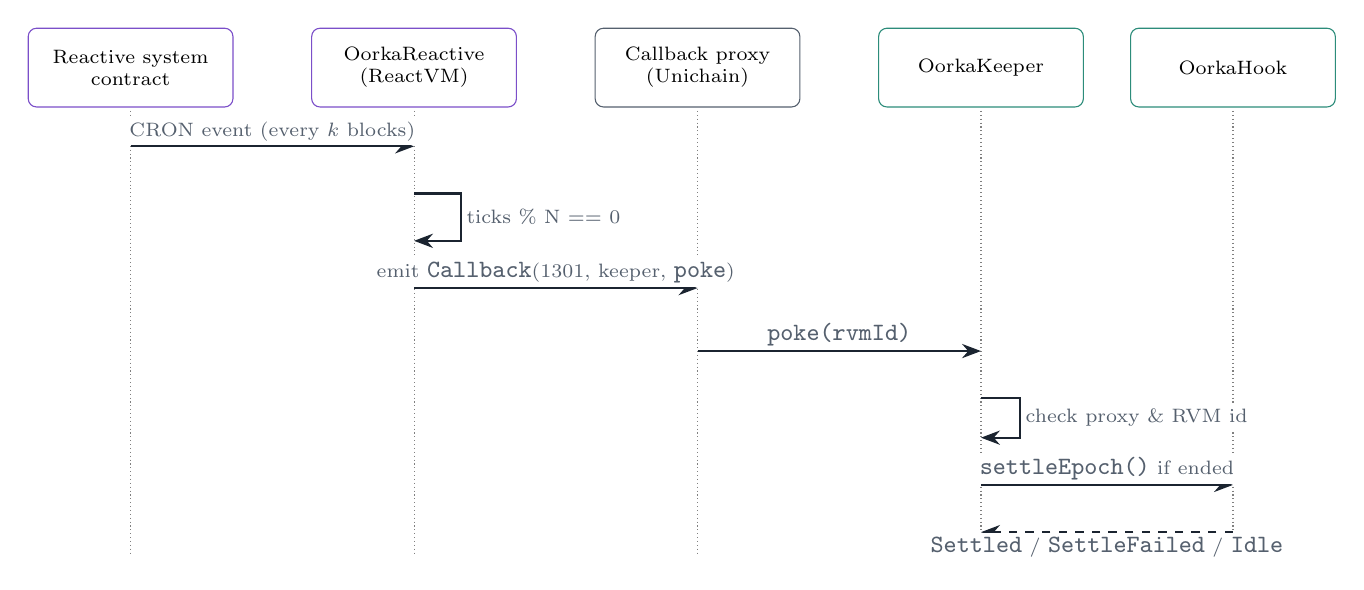
\begin{tikzpicture}[x=1cm,y=1cm]
  \foreach \x/\name/\col in {0/Reactive system\\contract/violet, 3.6/OorkaReactive\\(ReactVM)/violet, 7.2/Callback proxy\\(Unichain)/ink2, 10.8/OorkaKeeper/accent, 14.0/OorkaHook/accent}{
    \node[box,draw=\col,minimum width=2.6cm,font=\scriptsize] at (\x,0) {\name};
    \draw[densely dotted,color=gray] (\x,-0.55) -- (\x,-6.2);
  }
  \draw[arr] (0,-1.0) -- node[lbl,above]{CRON event (every $k$ blocks)} (3.6,-1.0);
  \draw[arr] (3.6,-1.6) -- ++(0.6,0) |- node[lbl,right,pos=0.25]{ticks \% N == 0} (3.6,-2.2);
  \draw[arr] (3.6,-2.8) -- node[lbl,above]{emit \code{Callback}(1301, keeper, \code{poke})} (7.2,-2.8);
  \draw[arr] (7.2,-3.6) -- node[lbl,above]{\code{poke(rvmId)}} (10.8,-3.6);
  \draw[arr] (10.8,-4.2) -- ++(0.5,0) |- node[lbl,right,pos=0.25]{check proxy \& RVM id} (10.8,-4.7);
  \draw[arr] (10.8,-5.3) -- node[lbl,above]{\code{settleEpoch()} if ended} (14.0,-5.3);
  \draw[darr] (14.0,-5.9) -- node[lbl,below]{\code{Settled} / \code{SettleFailed} / \code{Idle}} (10.8,-5.9);
\end{tikzpicture}}
\caption{Settlement automation. The reactive contract counts CRON ticks and sends a cross-chain callback. The keeper accepts calls only from the callback proxy carrying its own reactive contract's RVM id. A failed settle is reported and retried on the next tick, so the schedule can't get stuck.}
\label{fig:reactive}
\end{figure}

\subsection{Oorka Pulse: event-driven settlement}
A timer is a blunt instrument: with a 17-minute CRON tick and 15-minute epochs, an ended epoch can wait up to a full tick before the seat changes hands, and a vault move deferred during a price push waits just as long. \emph{Oorka Pulse} is a second reactive contract that listens to the pool instead of the clock. It subscribes on Unichain Sepolia to the PoolManager's \code{Swap} events filtered to Oorka's \code{PoolId}, and to the hook's \code{EpochSettled}, \code{VaultMoveDeferred} and \code{VaultMoved}.

\begin{itemize}
  \item \textbf{Epoch clock.} Pulse mirrors the hook's epoch end. Every \code{EpochSettled} sets $\textit{dueAt} \leftarrow t + T$.
  \item \textbf{Settle on time.} The first swap with $t \ge \textit{dueAt}$ requests a callback; the keeper calls \code{settleEpoch()}. Settlement lands seconds after the boundary.
  \item \textbf{Finish deferred moves.} \code{VaultMoveDeferred} raises a flag; the next swap requests a callback, and the keeper calls \code{compound()}, which moves the vault once the price is honest. \code{VaultMoved} clears the flag.
  \item \textbf{Safeguards.} A cooldown (30\,s) turns a burst of swaps into one callback. Logs from any other chain, pool or contract are ignored without reverting. Pulse calls the same keeper path anyone could, and the hook re-checks the epoch end and the price itself. The CRON contract keeps running as the fallback for quiet pools.
\end{itemize}

Each request emits \code{Triggered(reason, originBlock, originTx, n)}, which lets the full loop (origin swap $\rightarrow$ reactive transaction $\rightarrow$ callback) be measured from block timestamps on both chains. On the live deployment the first measured loop, from the origin swap to the keeper\'s \code{Settled} event, took 2 seconds; the CRON fallback alone can take up to 17 minutes.

\subsection{Liveness, not authority}
The keeper holds no privileged role on the hook: \code{settleEpoch()} is open to anyone. The keeper only adds \emph{liveness}, so the seat changes hands on time even when nobody is watching. A takeover settlement, which migrates the vault and re-marks every curator, uses under $1.5$M gas, half the $3$M callback budget. This bound is asserted in the tests.

% ====================================================================
\section{Implementation}
\subsection{Hook permissions and position layout}
Oorka requests exactly three permissions: \code{afterInitialize} (bind to a single pool, seed the price accumulator), \code{beforeSwap} (block-open snapshot and TWAP accumulation) and \code{beforeDonate} (reject donations). It never alters swap amounts or fees, so the pool remains an ordinary v4 pool for traders and routers.

\begin{table}[H]
\centering\small
\begin{tabular}{@{}lll@{}}
\toprule
\textbf{Position} & \textbf{Salt} & \textbf{Liquidity} \\
\midrule
Curator $i$ probe & \code{bytes32(i)} & $10^9$ at the declared range \\
Vault & \code{bytes32(type(uint256).max)} & depositor capital at the incumbent's range \\
\bottomrule
\end{tabular}
\caption{Hook-owned positions inside the PoolManager.}
\end{table}

\subsection{Core interface}
\begin{table}[H]
\centering\small
\begin{tabularx}{\linewidth}{@{}l l X@{}}
\toprule
\textbf{Function} & \textbf{Caller} & \textbf{Effect} \\
\midrule
\code{register(name, lo, hi, bond)} & anyone & Join with a bond and probe; the first registrant takes the seat. \\
\code{declareRange(id, lo, hi)} & curator & Move range (switch cost). If incumbent, the vault moves too. \\
\code{exit(id)} & challenger & Remove probe, reclaim bond. \\
\code{settleEpoch()} & anyone / keeper & Score, update streaks, take over if earned, roll baselines. \\
\code{deposit / withdraw} & depositor & Mint/burn shares priced at the block-open price. \\
\code{registerBenchmark(name, lo, hi)} & anyone, once & Fixed passive reference portfolio. \\
\code{benchmarkReport()} & view & Vault vs benchmark, since start and this epoch. \\
\code{settleSqrtPrice()} & view & Epoch TWAP price used at settlement. \\
\bottomrule
\end{tabularx}
\caption{Principal entry points of \code{OorkaHook}.}
\end{table}

\subsection{Settlement in pseudocode}
\begin{algorithm}[H]
\caption{\code{settleEpoch}}
\begin{algorithmic}[1]
\Require block.timestamp $\ge$ epochStart $+ T$
\State $\bar P \gets \textsc{EpochTwap}()$
\For{each active portfolio $i$}
  \State \textsc{MarkFees}$(i)$; \quad $G_i \gets \NAV_i(\bar P) / \NAV_i^{\text{start}}$
\EndFor
\State emit \textsc{BenchmarkScored}$(G_{\text{vault}}(\bar P),\, G_{\text{bench}})$
\State \textsc{ChargePerformanceFee}$(h)$ \Comment{mint $\phi$ of value above $\max(1, G_{\text{bench}}, \text{HWM})$}
\State $best \gets \bot$
\For{each challenger $i \ne h$, $i$ not benchmark}
  \If{joined before epoch \textbf{and} $G_i > G_h (1 + m)$} \State streak$_i \gets$ streak$_i + 1$
  \Else \State streak$_i \gets 0$ \EndIf
  \If{streak$_i \ge W$ \textbf{and} $G_i > G_{best}$} \State $best \gets i$ \EndIf
\EndFor
\If{$best \ne \bot$}
  \State slash $\sigma \cdot$ bond$_h$ into vault; reset all streaks; $h \gets best$
  \State \textsc{MigrateVault}(range$_{best}$)
\EndIf
\State roll all baselines at $\bar P$; update high-water mark; epoch $\gets$ epoch $+1$; snapshot accumulator
\end{algorithmic}
\end{algorithm}

\subsection{Parameters}
\begin{table}[H]
\centering\small
\begin{tabular}{@{}llr@{}}
\toprule
\textbf{Parameter} & \textbf{Meaning} & \textbf{Demo value} \\
\midrule
$T$ & epoch length & 10 min (local and testnet) \\
$W$ & consecutive wins needed for takeover & 2 \\
$m$ & margin over incumbent growth & 10 bps \\
$s$ & paper switch cost per range change & 30 bps \\
$\sigma$ & share of deposed bond paid to depositors & 20\% \\
$\phi$ & seat holder's performance fee above the hurdle & 10\% \\
$\delta_{\max}$ & max spot vs block-open deviation for vault actions & 300 ticks \\
min bond & minimum challenger bond & 100 token1 \\
$\NAV_0$ & paper portfolio notional & 1{,}000 token1 \\
$L_p$ & probe liquidity & $10^9$ \\
\bottomrule
\end{tabular}
\caption{Configuration. All values are constructor parameters.}
\end{table}

% ====================================================================
\section{Evaluation}\label{sec:eval}
\subsection{Test suite}
The Foundry suite has 61 tests and 5 invariants: 31 unit and 2 fuzz tests for the hook, 13 for the CRON keeper, 15 for Oorka Pulse, and a stateful invariant suite. It runs against a real v4 \code{PoolManager}, and continuous integration builds the contracts and runs every test on each push.
\begin{itemize}
  \item \textbf{Performance fee:} paid when the vault beats the benchmark, with depositors keeping 90\% of the excess; no fee when the benchmark wins; no fee on a flat epoch.
  \item \textbf{Measurement:} probes measure fees without capital; tight ranges out-earn wide ones in ranging markets; wide ranges win trending markets; out-of-range challengers never win.
  \item \textbf{Mechanism:} takeover after $W$ wins; vault migration; slashing to depositors; streak resets.
  \item \textbf{Benchmark:} starts flat; can't be moved, exited or seated; tracks the vault; uses no curator slot.
  \item \textbf{Manipulation:} in-block price pushes are ignored; donations revert with the exact wrapped error; a cross-block push leaves the settlement price near fair; a sustained move held for half the epoch counts for half.
  \item \textbf{Keeper:} no-op mid-epoch; settles ended epochs; drives a full takeover alone; rejects foreign callers and foreign RVM ids; settlement fits within half the callback gas budget.
  \item \textbf{Oorka Pulse:} silent mid-epoch; the first swap after the boundary requests exactly one callback; the full loop settles at the boundary; cooldown against bursts; deferred moves finished by \code{compound()}; foreign pools, chains and contracts ignored.
  \item \textbf{Invariants:} under random trades, deposits, withdrawals, curator churn and settlements, the hook stays solvent, the vault's books match the PoolManager, the curator array stays bounded, there is exactly one seat holder, and every probe sits at its declared range.
  \item \textbf{Accounting:} deposit/withdraw round trips (and a fuzzed version that can never create value); access-control reverts.
\end{itemize}

\subsection{Local demonstration}
A one-command demo deploys the full system on a local chain: a tETH/tUSD pool at about 3{,}000, background liquidity, and three seeded curators. Passive Pam ($\pm 40\%$) holds the seat; Tight Tony ($\pm 3\%$) and Mid Mia ($\pm 10\%$) challenge. A fixed benchmark sits at roughly $-50\%/+50\%$. Under range-bound order flow, Tony out-earned Pam in epochs~1 and~2 and took the seat at the end of epoch~2. Figure~\ref{fig:demo} shows the benchmark reports from that run.

\begin{figure}[h]
\centering
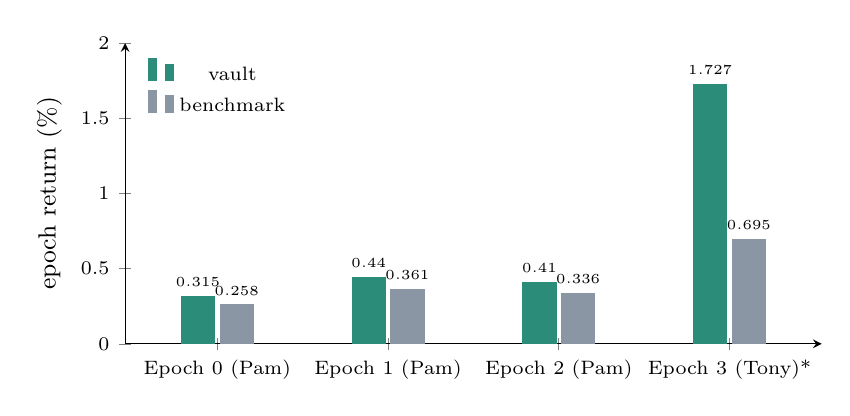
\begin{tikzpicture}
\begin{axis}[
  ybar, bar width=12pt, width=0.86\linewidth, height=5.4cm,
  symbolic x coords={E0,E1,E2,E3}, xtick=data,
  xticklabels={Epoch 0 (Pam),Epoch 1 (Pam),Epoch 2 (Pam),Epoch 3 (Tony)*},
  ylabel={epoch return (\%)}, ymin=0, ymax=2.0,
  nodes near coords, nodes near coords style={font=\tiny,/pgf/number format/fixed,/pgf/number format/precision=3},
  legend style={draw=none,font=\scriptsize,at={(0.02,0.97)},anchor=north west},
  tick label style={font=\scriptsize}, label style={font=\small},
  axis lines=left, enlarge x limits=0.18,
  ]
  \addplot[fill=accent,draw=accent] coordinates {(E0,0.315) (E1,0.440) (E2,0.410) (E3,1.727)};
  \addlegendentry{vault}
  \addplot[fill=bench,draw=bench] coordinates {(E0,0.258) (E1,0.361) (E2,0.336) (E3,0.695)};
  \addlegendentry{benchmark}
\end{axis}
\end{tikzpicture}
\caption{Vault vs benchmark per epoch in the local demo, from on-chain \code{BenchmarkScored} events. *Epoch~3 is the running epoch after Tony's takeover, read from \code{benchmarkReport()}. Since inception the vault returned $+2.96\%$ against the benchmark's $+1.66\%$. These are illustrative numbers from a synthetic market, not a performance claim.}
\label{fig:demo}
\end{figure}

\subsection{Regime change}
When the market trends (the demo's \emph{Pump tETH} action), price leaves Tony's $\pm3\%$ range. His probe stops earning fees and his portfolio sits fully in one token, so the wide-range curators lead the next epoch. If the trend persists for $W$ epochs, the seat moves back. No vote or operator is involved: the market regime itself decides who should manage.

% ====================================================================
\section{Testnet deployment}\label{sec:deploy}
Oorka runs on \textbf{Unichain Sepolia} (chain 1301) against the canonical Uniswap~v4 \code{PoolManager}, with its reactive contract on \textbf{Reactive Lasna} (chain 5318007). The deployment uses real testnet assets, Circle's USDC and the canonical WETH, and seeds the pool with three curators, the benchmark and a vault deposit, with $T = 15$ minutes. A market maker trading its own USDC and WETH moves the price through slow waves four times an hour so curators have real flow to be scored on.

\begin{table}[H]
\centering\small
\begin{tabularx}{\linewidth}{@{}l X@{}}
\toprule
\textbf{Contract} & \textbf{Address} \\
\midrule
\code{OorkaHook} (hook, vault, registry) & \href{https://sepolia.uniscan.xyz/address/0xd3F75e4DF6d0Cd75B17B66d577216f1F0630d0A0}{\texttt{\footnotesize 0xd3F75e4DF6d0Cd75B17B66d577216f1F0630d0A0}} \\
\code{OorkaPulse} (Lasna, event-driven) & \href{https://lasna.reactscan.net/address/0x0ee3b94d3eaa4b99c8c9840f3ab6139bbd9633aa}{\texttt{\footnotesize 0x0ee3b94d3eaa4b99c8c9840f3ab6139bbd9633aa}} \\
\code{OorkaKeeper} (Pulse callbacks) & \href{https://sepolia.uniscan.xyz/address/0x6716dad1ad8a91ce35b368466948d25efe48e3ee}{\texttt{\footnotesize 0x6716dad1ad8a91ce35b368466948d25efe48e3ee}} \\
\code{OorkaReactive} (Lasna, Cron1000 fallback) & \href{https://lasna.reactscan.net/address/0xdf4a40dd91683a72cea16175b40bbba2d9b48a3e}{\texttt{\footnotesize 0xdf4a40dd91683a72cea16175b40bbba2d9b48a3e}} \\
\code{OorkaKeeper} (CRON callbacks) & \href{https://sepolia.uniscan.xyz/address/0x75f6f1d2d9e3f0d321cccdf8502d9813df4d3241}{\texttt{\footnotesize 0x75f6f1d2d9e3f0d321cccdf8502d9813df4d3241}} \\
Uniswap v4 \code{PoolManager} & \href{https://sepolia.uniscan.xyz/address/0x00b036b58a818b1bc34d502d3fe730db729e62ac}{\texttt{\footnotesize 0x00b036b58a818b1bc34d502d3fe730db729e62ac}} \\
USDC (Circle) / WETH & \texttt{\footnotesize 0x31d0220469e10c4E71834a79b1f276d740d3768F} / \texttt{\footnotesize 0x4200000000000000000000000000000000000006} \\
\bottomrule
\end{tabularx}
\caption{Live contracts. Explorer links: Uniscan (Unichain Sepolia) and Reactscan (Lasna).}
\label{tab:deploy}
\end{table}

\paragraph{Dashboard.} The app at \href{https://oorka.djyo.tech}{\texttt{oorka.djyo.tech}} (documentation at \href{https://oorkadocs.djyo.tech}{\texttt{oorkadocs.djyo.tech}}) reads the testnet deployment. Users connect a browser wallet to register as curators, deposit, trade, and settle epochs. The same frontend runs against a local chain for the scripted demo.

\paragraph{Status (27 November 2026).} Every ended epoch since deployment has been settled without a human transaction. Oorka Pulse settles epochs within seconds of the first swap after the boundary; the CRON contract covers the rest. Both reactive contracts run with zero debt.

% ====================================================================
\section{Related work}
\begin{itemize}
  \item \textbf{Auction-managed AMMs}~\cite{amamm} auction the right to set fees and capture arbitrage, paying rent to LPs. Public hook implementations include Chronus (strategists compete on volatility forecasts), Maestro (autonomous Reactive manager) and Turnstile (anti-entrenchment throttle). These allocate the seat by \emph{willingness to pay}; Oorka allocates it by \emph{measured LP performance}.
  \item \textbf{Automated range managers} rebalance a fixed strategy, often with keepers or Reactive callbacks. They manage liquidity, but they don't let competing strategies prove themselves or replace each other.
  \item \textbf{LP tournaments and leaderboards} reward the best performers with prizes, but don't move depositor capital to the winner.
\end{itemize}

% ====================================================================
\section{Limitations and future work}
\begin{itemize}
  \item \textbf{Wash trading} remains costly but possible. Next: per-epoch fee-credit caps, or weighting by distinct swappers.
  \item \textbf{Single vault per pool.} Next: several vaults with different risk mandates reading one leaderboard.
  \item \textbf{Unmatched migration remainder} stays idle. Next: swap-based rebalancing on migration through the pool's own liquidity.
  \item \textbf{Single benchmark.} The hurdle is one fixed wide range. Next: let governance or depositors choose among several passive benchmarks, or a volatility-adjusted one.
  \item \textbf{Testnet liveness.} At the time of writing, CRON callbacks from Lasna had not yet reached the keeper on Unichain Sepolia (Section~\ref{sec:deploy}). Settlement stays permissionless, so anyone can still call \code{settleEpoch()}.
\end{itemize}

% ====================================================================
\section{Conclusion}
Oorka replaces ``trust the manager'' with ``the manager is whoever is measurably winning''. Dust probe positions let Uniswap~v4 measure any strategy on live order flow. A small, auditable state machine turns those measurements into automatic manager selection and liquidity migration. A hook-built TWAP, block-open accounting and donation rejection make the measurements hard to game. A passive benchmark tells depositors, every epoch, whether active curation was worth it, and the manager is paid only for the part that was. Reactive Network keeps the whole loop running without an operator, and Oorka Pulse closes each epoch seconds after it ends.

% ====================================================================
\begin{thebibliography}{9}\small
\bibitem{univ3} H.~Adams, N.~Zinsmeister, M.~Salem, R.~Keefer, D.~Robinson. \emph{Uniswap v3 Core}. 2021.
\bibitem{univ4} H.~Adams et al. \emph{Uniswap v4 Core}. 2024. \url{https://github.com/Uniswap/v4-core}
\bibitem{lvr} J.~Milionis, C.~C.~Moallemi, T.~Roughgarden, A.~L.~Zhang. \emph{Automated Market Making and Loss-Versus-Rebalancing}. 2022.
\bibitem{amamm} A.~Adams, C.~C.~Moallemi, S.~Reynolds, D.~Robinson. \emph{am-AMM: An Auction-Managed Automated Market Maker}. 2024.
\bibitem{reactive} Reactive Network documentation. \url{https://dev.reactive.network}
\bibitem{uhidir} Atrium Academy. \emph{UHI Hook Directory}. \url{https://atriumacademy.notion.site/hook-directory}
\end{thebibliography}

\end{document}
